\documentclass[12pt,a4paper]{article}
\usepackage{preamble} % preamble.sty
% -----------------------------------------------------------------


\begin{document}
% Титульная страница (файл title.tex)
\begin{titlepage}
	\centering
	
	{\Large Санкт-Петербургский Государственный Университет \par}
	
	\vspace{0.5cm}
	
	{\large Факультет математики и механики\par}
	
	\vspace{7.5cm}
	
	{\Huge\bfseries Теория вероятностей} % Название

        \vspace{0.3cm}
	
        {\large Лектор: Зайцев~А.~Ю.}
        
        \vspace{1cm}
        
        {\Large 5 семестр}


\end{titlepage}
% Содержание
\tableofcontents
\newpage
% - - - - - - - - - - - - - - - - - -

\section{Лекция 02.09.25}
В средние века довольно популярной была игра в кости. На гранях кубика изображены числа из множества $\{1, 2, 3, 4, 5, 6\}$. Если предположить, что кубик идеален (т.е. симметричен и однороден), и подбрасывается в идеальных условиях без посторонних воздействий, то у нас нет объективных причин считать одну грань более предпочтительной, чем другую. Такие элементарные исходы являются равновозможными.

В таком случае, вероятность выпадения любой конкретной грани, например, шестёрки, определяется как отношение числа благоприятствующих исходов к общему числу всех возможных равновероятных исходов: $\mathbb{P}(\text{``выпала шестёрка''}) = \frac{1}{6}.$

Аналогично, вероятность события ``выпало чётное число'' (исходы: $2, 4, 6$) будет равна: $\mathbb{P}(\text{``чётное число''}) = \frac{3}{6} = \frac{1}{2}.$

Это классическое определение вероятности, которое эффективно, когда пространство исходов конечно и исходы равновозможны. Однако для более сложных задач (бесконечные пространства, неравновозможные исходы) потребуется более общий аксиоматический подход.

\begin{remind}
Комбинаторика предоставляет инструменты для подсчёта числа исходов, что часто помогает в вычислении вероятностей по классическому определению:
\begin{itemize}
    \item Число перестановок из $n$ различных элементов: $$n!$$
    \item Размещения: Число способов выбрать $k$ элементов из $n$ (порядок важен): $$A_n^k = \frac{n!}{(n-k)!}$$
    \item Сочетания: Число способов выбрать $k$ элементов из $n$ (порядок не важен): $$C_n^k = \binom{n}{k} = \frac{n!}{k! \cdot (n-k)!}$$
\end{itemize}
\end{remind}

\begin{definition}[Колмогоровская модель]
    \textit{Вероятностное пространство} -- тройка $\left( \Omega, \mathcal{F}, \mathbb{P} \right)$, где \begin{itemize}
        \item $\Omega$ -- множество элементарных исходов;
        \item $\mathcal{F}$ -- $\sigma$-алгебра подмножеств $\Omega$ ($\sigma$-алгебра событий);
        \item $\mathbb{P}$ -- вероятностная мера на $\mathcal{F}$, то есть функция $\mathbb{P} : \mathcal{F} \to [0, 1]$ такая, что \begin{enumerate}
        \item $\mathbb{P}(A) \geq 0$ (неотрицательность);
        \item $\mathbb{P}(\Omega) = 1$ (нормированность);
        \item $A_1, \ldots, A_n, \ldots \text{ и } A_i \cap A_j = \varnothing$, тогда $\mathbb{P}\left( \bigcup\limits_{i = 1}^{\infty} A_i \right) = \sum\limits_{i=1}^{\infty} \mathbb{P}(A_i)$ (счетная аддитивность).
    \end{enumerate}
    \end{itemize} 
\end{definition}

\begin{remark}
    Дискретная модель вкладывается в колмогоровскую, если взять в качестве $\sigma$-алгебры все подмножества $\Omega$.
\end{remark}

\begin{definition}
    Событие единичной вероятности называется \textit{достоверным}.
\end{definition}

\begin{definition}
    Событие нулевой вероятности называется \textit{невозможным}.
\end{definition}

\begin{example}
    Если мы бросаем шарик в квадратную область, то вероятность попасть в какую-то конкретную точку равна нулю, потому что мера Лебега точки равна нулю.
\end{example}

\begin{definition}
    \textit{Геометрическая вероятность} — модель, где вероятностное пространство $\Omega$ является измеримым подмножеством $\mathbb{R}^n$ с мерой Лебега $\lambda$, причём $0 < \lambda(\Omega) < +\infty$. Вероятность определяется как нормированная мера Лебега: $$\mathbb{P}(A) = \frac{\lambda(A)}{\lambda(\Omega)}, \qquad A \subset \Omega, \; A \in \mathcal{B}.$$ В этом случае часто рассматривают борелевскую $\sigma$-алгебру $\mathcal{B}$ (наименьшау $\sigma$-алгебру, которая содержит все открытые множества $\Omega$). 
\end{definition}

\begin{example}
    На плоскости задан прямоугольник со сторонами $a, b > 0$. С какой вероятностью случайно выбранная в нем точка будет ближе к центру прямоугольника, чем к любому из его углов?
\end{example}
\begin{solution}
    Множество искомых точек в общем случае образует неправильный шестиугольник (см. Рис. \ref{fig:ex1}).
\end{solution}

\begin{figure}[h]
    \centering
    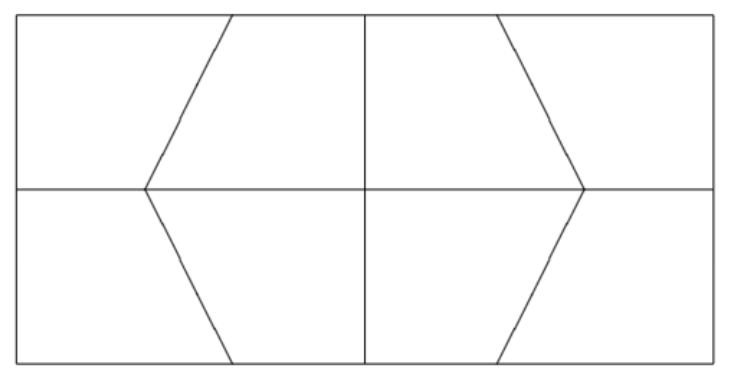
\includegraphics[scale=0.3]{images/ex1.png}
    \caption{Множество искомых точек}
    \label{fig:ex1}
\end{figure}

\begin{definition}
    Пусть $A, B \in \mathcal{F},$ тогда $A, B$ называют \textit{совместными}, если $A \cap B \neq \varnothing$.
\end{definition}

\begin{example}
При подбрасывании игрального кубика:
\begin{itemize}
    \item Событие $A$: ``выпало четное число'' $\{2, 4, 6\}$;
    \item Событие $B$: ``выпало число, меньшее 3'' $\{1, 2\}$;
\end{itemize}
Они совместные, так как $A \cap B = \{2\}$ (исход ``2'' благоприятствует обоим событиям).
\end{example}

\begin{definition}
    \textit{Условная вероятность} события $A$ при условии наступления события $B$ определяется формулой: $$\mathbb{P}\left( A \mid B \right) = \frac{\mathbb{P}\left( A \cap B \right)}{\mathbb{P}\left( B \right)}, \qquad \text{если } \mathbb{P}\left(B\right) \neq 0.$$
\end{definition}

\section{Лекция 09.09.25}

Используя формулу для условной вероятности, переписанную в виде \[ \mathbb{P} \left( A \cap B\right) = \mathbb{P} \left( A \mid B\right) \cdot \mathbb{P} \left( B\right) = \mathbb{P} \left( B \mid A\right) \cdot \mathbb{P} \left( A\right),\]
можно по индукции доказать, что: \[ \mathbb{P} \left( A_1 \cap A_2 \cap \dots \cap A_n \right) = \mathbb{P} \left( A_1 \right) \cdot \mathbb{P} \left( A_2 \mid A_1 \right) \cdot \ldots \cdot \mathbb{P}\left(A_n \mid A_1 \cap \dots \cap A_{n-1}\right).\]

\begin{definition}
    События \(A_1, \ldots, A_n \) называют \textit{независимыми в совокупности}, если вероятность пересечения любого числа событий будет равна произведению вероятностей каждого отдельного события, в частности: \[ \mathbb{P} \left(A_1 \cap \dots \cap A_n\right) = \mathbb{P} \left( A_1\right) \cdot \ldots \cdot \mathbb{P} \left( A_n\right);\]
\end{definition}

\begin{remark}
    Если \(A, B\) - независимые, то \(A, \overline{B}\) - тоже независымые.
\end{remark}

Используя это замечание, можно получить, что: \( \mathbb{P}( A \cap \overline{B}) = \mathbb{P} ( A) \cdot \mathbb{P} ( \overline{B})= \mathbb{P}( A) ( 1 - \mathbb{P}( B)) = \mathbb{P}( A) - \mathbb{P}( A) \mathbb{P}( B) = \mathbb{P}(A) - \mathbb{P}( A \cap B).\)

Рассмотрим теперь \(\Omega = H_1 \sqcup \dots \sqcup H_n\). 

\begin{definition}
    Такой набор \(H_1, \ldots, H_n\) называт \textit{полной группой несовместных событий}, а каждое конкретное \(H_j\) - \textit{гипотезой}. 
\end{definition}

Возьмем \(A \in \mathcal{F}\) и распишем его используя полную группу гипотез: \( A = (H_1 \cap A) \cup (H_2 \cap A) \cup \dots (H_n \cap A)\), получили объединение попарно непересекающихся множеств.
Очевидным образом получим: \(\mathbb{P} (A) = \mathbb{P}(H_1 \cap A) + \ldots + \mathbb{P} (H_n \cap A).\)

Теперь воспользуемся переписанной формулой условной вероятности: \(\mathbb{P}(H_j \cap A) = \mathbb{P} (H_j) \cdot \mathbb{P}(A \mid H_j).\)
В итоге получаем:

\begin{definition}[Формула полной вероятности]
    \[\mathbb{P}(A) = \sum\limits_{ i = 1}^{n} \mathbb{P} (H_j) \mathbb{P} (A \mid H_j);\]
\end{definition}

Теперь найдем \(\mathbb{P}(H_j \mid A)\). Воспользуемся формулой условной вероятности: \( \mathbb{P}(H_j \mid A) = \frac{ \mathbb{P} (H_j \cap A)}{ \mathbb{P}(A)},\) при условии, что \(\mathbb{P}(A) \neq 0\). Распишем числитель, используя переписанную формулу условной вероятности, а для знаменателя воспользуемся формулой полной вероятности: 

\begin{definition}[Формула Байеса]
    \[\mathbb{P}(H_j \mid A) = \frac{\mathbb{P} (H_j) \mathbb{P} (A \mid H_j)}{ \sum\limits_{i = 1}^{n} \mathbb{P}(H_i) \mathbb{P}(A \mid H_i)}.\]
\end{definition}

\begin{example}
    Представим, что на некотором заводе работает \(3\) станка \((H_1, H_2, H_3)\), производящих детали. Эти детали могут быть бракованными. 
    Мы случайным образом берем одну произведенную на заводе деталь. Событие \(A\) будет состоять в том, что деталь, которую мы взяли оказалась бракованной. Нам известно с какой вероятностью каждый из станков производит бракованные детали, а также известна их производительность.
    Пусть \(\mathbb{P}(H_1) = 0.4, \; \mathbb{P}(H_2) = 0.35, \; \mathbb{P}(H_3) = 0.25, \; \mathbb{P}(A \mid H_i) = 0.03.\) Оказалось, что взятая нами деталь бракованная. Требуется понять с какой вероятностью она была произведена на станке под номером \(1\).

\end{example}

\begin{example}
    Еще пример, про болезнь и результат теста.
\end{example}

\begin{definition}
    \textit{Случайная величина} --- измеримая функция из \(\Omega\) в \(\mathbb{R}\): \[\xi : \Omega \to \mathbb{R}, \; \; \xi^{-1}(B) \in \mathcal{F} \;\; \forall B \in \mathcal{B} \text{ (} \sigma \text{-алгебра борелевских подмножеств } \Omega \text{)}.\]
\end{definition}

\begin{remark}
    Зачем нужна измеримость? Потому что мы будем интересоваться вероятностями событий вида \(\mathbb{P}(\xi \in B)\), то есть \(\mathbb{P}\left\{ \omega : \xi(\omega) \in B\right\}\) а они существуют только если \(\xi^{-1}(B)\) лежит в \(\sigma\)-алгебре \(\mathcal{F}\), так как вероятность определена только на ней. Так что это минимальное требование к функции -- быть измеримой.
\end{remark}

\begin{definition}
    Если \(\xi : \Omega \to \mathbb{R}\) -- случайная величина, то с ней можно связать \textit{распределение случайной величины} --- вероятнострую меру на \(\mathcal{B}\): \[P_{\xi}(B) = \mathbb{P}(\xi \in B), \; \; B \in \mathcal{B};\]
\end{definition}

\begin{remark}
    Другими словами, если для случайной величины \(\xi\) мы знаем \(\mathbb{P}(\xi \in B)\), то мы знаем ее распределение.
\end{remark}

\begin{definition}
    \textit{Схемой Бернулли} называется вероятностный эксперимент, удовлетворяющий следующим условиям:

\begin{enumerate}
    \item Проводится серия из $n$ последовательных \textit{независимых} испытаний.
    \item Каждое испытание имеет ровно \textit{два исхода}: условно называемые \textit{``успех''} (событие $A$) и \textit{``неудача''} (событие $\overline{A}$, дополнение к $A$).
    \item \textit{Вероятность «успеха»} в каждом отдельном испытании \textit{постоянна} и равна $p$, где $0 \leq p \leq 1$. Соответственно, вероятность ``неудачи'' равна $q = 1 - p$.
\end{enumerate}
Формализация с помощью индикаторной случайной величины: для математического описания $k$-го испытания в серии ($k = 1, 2, \dots, n$) вводится \textit{индикаторная случайная величина} $\xi_k$:

\[
\xi_k(\omega) = 
\begin{cases}
1, & \text{если } \omega \in A, \\
0, & \text{если } \omega \notin A .
\end{cases}
\]
Эта величина имеет \textit{распределение Бернулли} с параметром $p = \mathbb{P}(A)$:
\[
P_{\xi}(x) = 
\begin{cases}
p, & \text{при } x = 1, \\
1 - p, & \text{при } x = 0.
\end{cases}
\]
\end{definition}

\begin{example}[Геометрическая модель схемы Бернулли для \(n = 2\)]
    Для наглядного представления последовательности из двух независимых испытаний Бернулли используется модель с единичным квадратом. Пространство элементарных исходов: \( \Omega = [0, 1] \times [0,1]\). Каждая точка \(\omega = (\omega_1, \omega_2)\) -- это возможный исход всего опыта.

    Независимость обеспечена тем, что мы используем нормированную меру Лебега. Вероятность попадания в любое множество (событие) равна его площади, так как площадь всего \(\Omega\) равна \(1\). Это в точности соответствует правилу умножения вероятностей для независимых событий.
\end{example}

\begin{definition}
    Пусть \(\xi\) -- случайная величина, тогда \(F : \mathbb{R} \to \mathbb{R}\): \[F(x) = \mathbb{P}(\xi < x) = P_{\xi} ((- \infty , x]), \; \; x \in \mathbb{R}\] называется \textit{функцией распределения случайной величины} \(\xi\) (или меры \(P_{\xi}\)).
\end{definition}

\begin{remark}
    Функция распределения однозначно характеризует распределение.
\end{remark}

\begin{example}[Схема Бернулли]
    Функция распределения \(\xi_k\) имеет вид (см. Рис \ref{fig:ex2}): \[F_{\xi_{k}} (x) = \mathbb{P}(\xi_{k} \leq x) = \begin{cases}
        0, \; \; x < 0, \\
        1 - p,\;\; 0 \leq x < 1, \\
        1, \;\;x \geq 1.
    \end{cases}\]
\end{example}


\begin{figure}[h]
    \centering
    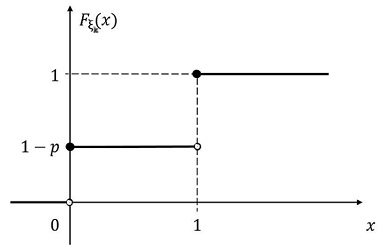
\includegraphics[scale=0.4]{images/ex2.png}
    \caption{График функции распределения для \(\xi_k\)}
    \label{fig:ex2}
\end{figure}


\section{Лекция 16.09.25}
hello

hello

hello

hello

hello
\end{document}